\documentclass{article}

\usepackage[utf8]{inputenc}
\usepackage[ngerman]{babel}
\usepackage[ngerman]{translator}
\usepackage[T1]{fontenc}
\usepackage{enumitem}
\usepackage{graphicx}
\usepackage{float}
\usepackage{url}
\usepackage[bottom]{footmisc}
\usepackage{hyperref}
\usepackage[nonumberlist, section=subsection]{glossaries}

\title{\textbf{Entwurf} \\ Cryptographics}
\author{}
\date{\today}

%Glossar-Befehle anschalten
\makeglossaries
% \newglossaryentry{identifier}{name={Name}, description={Description}}

\begin{document}

% The cover page.
\maketitle
\begin{table}[b]
  \begin{tabular}{| l | l | l |}
    \hline
    \textbf{Phase} & \textbf{Verantwortlicher} & \textbf{Email} \\ \hline
    Pflichtenheft & Matthias Jaenicke & matthias.jaenicke@student.kit.edu \\ \hline
    Entwurf & Matthias Plappert & undkc@student.kit.edu \\
            & Julien Duman & uncyc@student.kit.edu \\ \hline
    Implementierung & Christian Dreher & uaeef@student.kit.edu \\ \hline
    Qualitätssicherung & Wasilij Beskorovajnov & uajkm@student.kit.edu \\ \hline
    Präsentation & Aydin Tekin & aydin.tekin@student.kit.edu \\ \hline
    \end{tabular}
\end{table}
\thispagestyle{empty}
\newpage

% Table of contents page.
\tableofcontents
\newpage

% Start of the actual document.
\section{Einleitung}
Für das Kryptologikum des Instituts für Kryptographie und Sicherheit soll die Software Cryptographics zur Demonstration kryptographischer Verfahren erstellt werden. Das Softwareprodukt soll vor allem auf Ausstellungen präsentiert werden und erfordert daher eine möglichst intuitive Benutzerführung.

Um das Ziel der intuitiven Benutzerinteraktion zu erreichen, liegt das Hauptaugenmerk des Entwurfes auf der Planung eines Rahmenwerkes, dass es erlaubt, einzelne Verfahren in die Software einzubetten. Durch wiederverwendbare UI-Komponenten sowie eine einheitliche und für alle Verfahren identischen Benutzerführung erreichen wir dieses Ziel. Zusätzlich erlaubt uns dieser Entwurf, wiederkehrende Aufgaben wie beispielsweise die Soforthilfe mit minimalem Aufwand innerhalb der einzelnen Verfahren zu implementieren. Die eigentliche Komplexität steckt hierbei immer im Rahmenwerk, sodass alle Verfahren von Verbesserungen und Optimierungen profitieren. Weiterhin setzen wir auf eine simples, modulares System, dass es uns erlaubt, Verfahren mit minimalem Aufwand zu implementieren, zu warten und auszutauschen. Grundprinzipien ist hierbei die lose Kopplung der einzelnen Verfahren.

Eine Herausforderung stellte die Abwägung zwischen Konsistenz und einer nötigen Flexibilität innerhalb der Verfahren da. So erfordern beispielsweise unterschiedliche Verfahren durchaus sehr unterschiedliche Arten der Navigation. Unser Entwurf sieht hierbei vor, dass die einzelnen Verfahren durchaus flexible und ohne strikte Vorgaben funktionieren können, gewisse Funktionen wie beispielsweise die Hilfe immer auf dieselbe Art funktionieren. Das oben beschriebene Rahmenwerk agiert auch hier unterstützend, erlaubt aber eine gewisse Flexibilität beispielsweise bei der Navigation innerhalb des Verfahrens. Somit lassen sich eine Vielzahl von unterschiedlichen Visualisierungen realisieren.

\section{Aufbau}

\subsection{Architektur}

Die grundlegende Architektur gliedert sich in 4 Schichten. Hierbei implementieren die Schichten von unten nach oben Funktionalität, die dann in der höheren Schicht verwendet werden kann.

\begin{figure}[H]
  \centering
    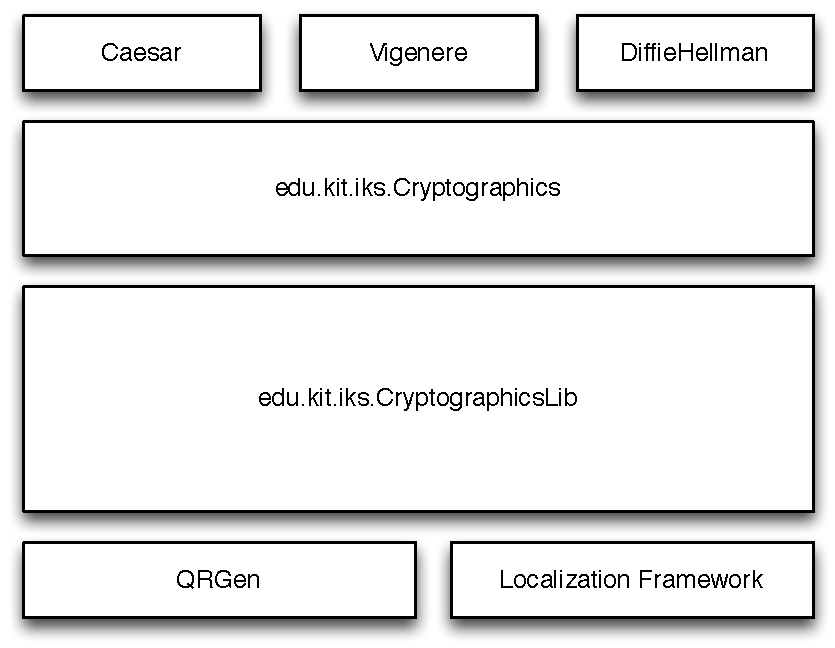
\includegraphics[width=\textwidth]{resources/architecture}
  \caption{Architekturübersicht.}
\end{figure}

In der ersten, der untersten Schicht befinden sich Bibliotheken von Drittanbietern. In unserem Fall handelt es sich hierbei um QRGen, eine Java-Bibliothek um QR-Codes zu generieren, sowie um ein Framework zur Lokalisierung.

In der zweiten Schicht befindet sich das Modul edu.kit.iks.CryptographicsLib. Dieses Modul enthält zum Einen abstrakte Klassen, die von den weiter oben liegenden Klassen verwendet werden. Zum Anderen finden sich hier wiederverwendbare UI-Komponenten, die beispielsweise bei verschiedenen Verfahren verwendet werden können.

Die dritte Schicht besteht aus dem Modul edu.kit.iks.Cryptographics. Hierbei handelt es sich um das Rahmenwerk, in dem alle Visualisierungen ausgeführt werden. Hier wird beispielsweise die Logik implementiert um zwischen Verfahren über eine Zeitleiste wechseln zu können oder auch die Soforthilfe.

Die oberste und vierte Schicht besteht aus den einzelnen, konkreten Verfahren.

Alle Schichten unterteilen ihre Klassen nach dem Model-View-Controller-Prinzip um eine Trennung von Datenmodell, Präsentation und Programmsteuerung zu erreichen. Sowohl die Präsentation als auch die Programmsteuerung verwendet hierbei das Entwurfsmuster Kompositum. Dies erlaubt es uns, eine hierarchische Struktur zu implementieren, und die Aufgaben der Programmsteuerung klar voneinander abzugrenzen. Eine schematische Darstellung der Controller-Hierarchie während einer Visualisierung ist in Abb. 2 zu finden.

\begin{figure}[H]
  \centering
    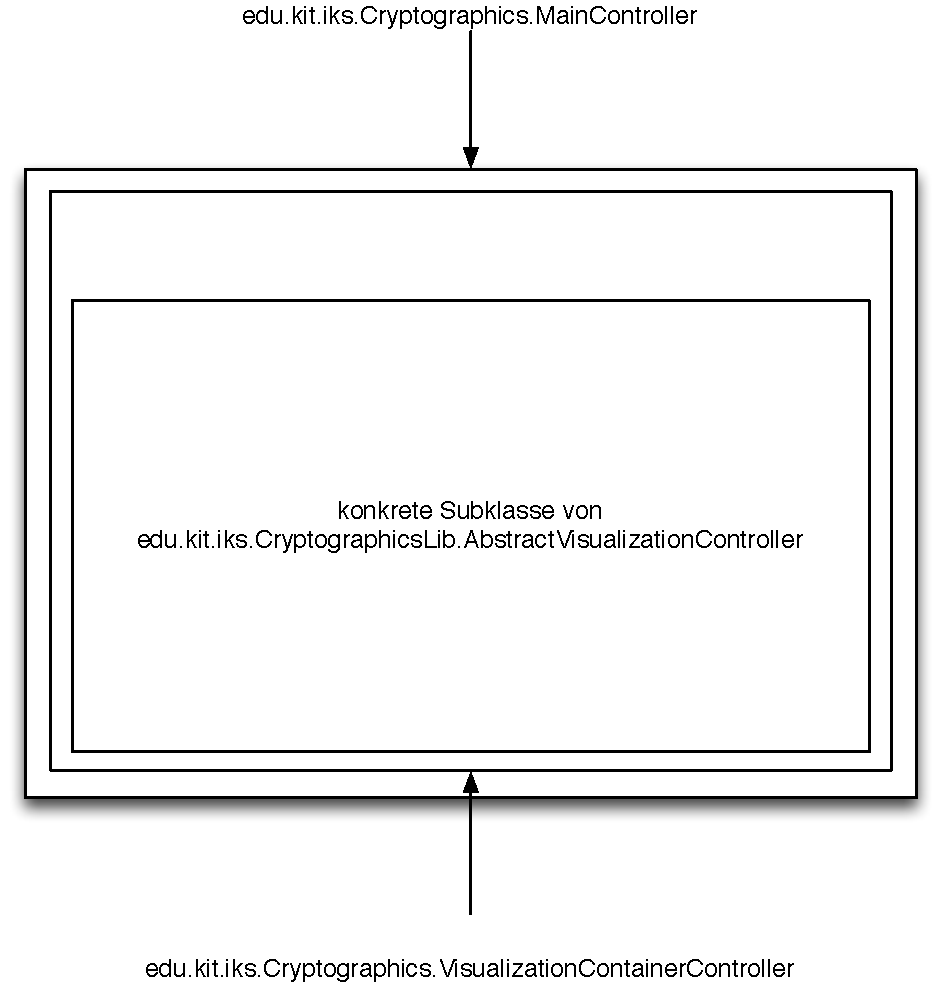
\includegraphics[width=\textwidth]{resources/architecture-2}
  \caption{Darstellung der einzelnen Controller während einer Visualisierung.}
\end{figure}

\section{Klassenbeschreibung}
  \subsection{Paket edu.kit.iks.Cryptographics}
    \subsubsection{Klasse MainController}
      Der MainController erzeugt das Fenster und verwaltet Start- und VisualizationContainerController.
      \begin{figure}[H]
        \centering
        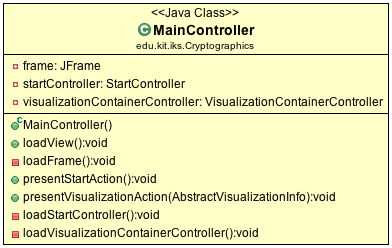
\includegraphics[width=\textwidth]{resources/edu-kit-iks-Cryptographics-MainController}
      \end{figure}

      \textbf{Superklassen und Interfaces}
      \begin{itemize}
        \item edu.kit.iks.CryptographicsLib.AbstractController
      \end{itemize}
      
      \textbf{Methoden}
      \begin{itemize}
        \item public void presentStartAction() \newline
        Lädt den StartController und zeigt seine View an.
      \end{itemize}

  \subsection{Paket edu.kit.iks.CryptographicsLib}
  	\subsection{Klasse AbstractController}
	  Um die MVC-Architektur zu erleichtern wird ein abstrakter Controller benötigt, mit dem Mechanismen
	  für die Controller ausgelagert werden können. Des Weiteren bietet das die Möglichkeit, konkrete
	  Controller mit Hilfe ihrer Substitution anzusprechen.
	
      \begin{figure}[H]
        \centering
        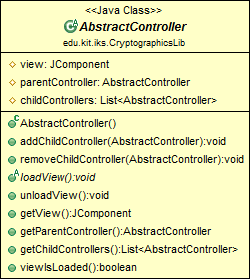
\includegraphics[width=\textwidth]{resources/edu-kit-iks-CryptographicsLib-AbstractController}
      \end{figure}
	
      \textbf{Superklassen und Interfaces}
      \begin{itemize}
        \item \textit{keine}
      \end{itemize}
	
      \textbf{Methoden}
      \begin{itemize}
        \item public void addChildController(AbstractController childController) \newline
          Fügt den übergebenen Kind-Controller zur Liste der Kind-Controller hinzu.
        
        \item public void removeChildController(AbstractController childController) \newline
          Entfernt den übergebenen Kind-Controller aus der Liste der Kind-Controller.
          
        \item abstract public void loadView() \newline
          Abstrakte Deklaration der loadView()-Methode zwingt die erbenden Controller dazu,
          zu definieren, wie ihre View geladen werden soll.
          
        \item public void unloadView() \newline
          Gibt den von der View verbrauchten Speicher wieder frei, sofern diese nicht mehr
          benötigt wird. Zu beachten ist, dass diese Methode über eine Standardimplementierung
          verfügt, es aber durchaus sinnvoll sein kann, das Standardverhalten durch eine
          eigene Implementierung zu überschreiben.
        
        \item public boolean viewIsLoaded() \newline
          Prüft ab, ob die View bereits geladen ist oder nicht.
      \end{itemize}
      
      \textbf{Getter}
      \begin{itemize}
        \item public JComponent getView()
        \item public AbstractController getParentController()
        \item public List<AbstractController> getChildControllers()
      \end{itemize}
      
      \textbf{Setter}
      \begin{itemize}
        \item \textit{keine}
      \end{itemize}
	
  \subsection{Paket edu.kit.iks.Cryptographics.Vigenere}
    \subsubsection{Klasse AbstractController}
      Der AbstractController ist eine abstrakte Klasse, die die verschiedenen State-Controller im Vigenere-Paket nutzen.
      \begin{figure}[H]
        \centering
        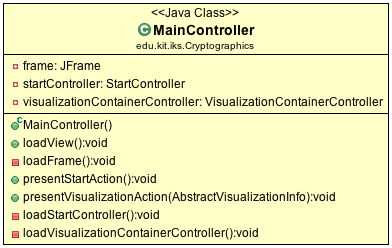
\includegraphics[width=\textwidth]{resources/edu-kit-iks-Cryptographics-MainController}
      \end{figure}

      \textbf{Superklassen und Interfaces}
      \begin{itemize}
        \item edu.kit.iks.CryptographicsLib.AbstractVisualizationController
      \end{itemize}
      
      \textbf{Methoden}
      \begin{itemize}
        \item public String getHelp() \newline
        Gibt den Hilfe-Text an.
        \item public String loadView() \newline
        Lädt die View zum zugehörigen Zustand.
      \end{itemize}

    \subsubsection{Klasse VigenereModel}
      Das VigenereModel ist für die Ver- und Entschlüsselung zuständig.
      \begin{figure}[H]
        \centering
        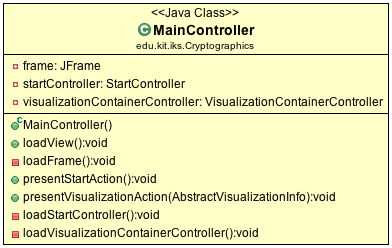
\includegraphics[width=\textwidth]{resources/edu-kit-iks-Cryptographics-MainController}
      \end{figure}
      
      \textbf{Methoden}
      \begin{itemize}
        \item public char XOR(char a, char b) \newline
        Benutzt einen logischen XOR auf die Parameter a und b.
      \end{itemize}

\subsection{Paket edu.kit.iks.Cryptographics.Caesar}
\subsection{Paket edu.kit.iks.Cryptographics.DiffieHellman}

\section{Abläufe}

\section{Entwurfdaten}

\section{Anhang}
\glsaddall
\printglossary[numberedsection, style=altlist]

\end{document}
